\section{moeo\-Fast\-Non\-Dominated\-Sorting\-Fitness\-Assignment$<$ MOEOT $>$::Objective\-Comparator Class Reference}
\label{classmoeoFastNonDominatedSortingFitnessAssignment_1_1ObjectiveComparator}\index{moeoFastNonDominatedSortingFitnessAssignment::ObjectiveComparator@{moeoFastNonDominatedSortingFitnessAssignment::ObjectiveComparator}}
Functor allowing to compare two solutions according to their first objective value, then their second, and so on.  


Inheritance diagram for moeo\-Fast\-Non\-Dominated\-Sorting\-Fitness\-Assignment$<$ MOEOT $>$::Objective\-Comparator::\begin{figure}[H]
\begin{center}
\leavevmode
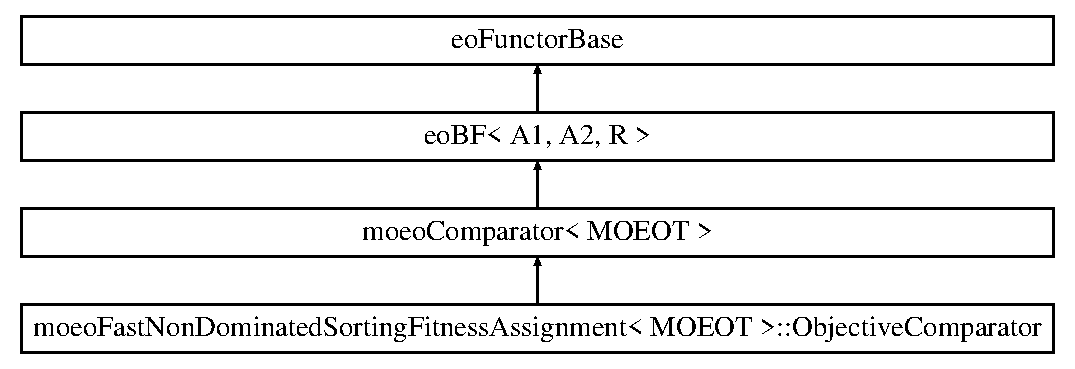
\includegraphics[height=4cm]{classmoeoFastNonDominatedSortingFitnessAssignment_1_1ObjectiveComparator}
\end{center}
\end{figure}
\subsection*{Public Member Functions}
\begin{CompactItemize}
\item 
const bool \bf{operator()} (const MOEOT \&\_\-moeo1, const MOEOT \&\_\-moeo2)
\begin{CompactList}\small\item\em Returns true if \_\-moeo1 $<$ \_\-moeo2 on the first objective, then on the second, and so on. \item\end{CompactList}\end{CompactItemize}
\subsection*{Private Attributes}
\begin{CompactItemize}
\item 
\bf{moeo\-Objective\-Objective\-Vector\-Comparator}$<$ \bf{Objective\-Vector} $>$ \bf{cmp}\label{classmoeoFastNonDominatedSortingFitnessAssignment_1_1ObjectiveComparator_2280f5d8df81b5c69676fa4fade67719}

\begin{CompactList}\small\item\em the corresponding comparator for objective vectors \item\end{CompactList}\end{CompactItemize}


\subsection{Detailed Description}
\subsubsection*{template$<$class MOEOT$>$ class moeo\-Fast\-Non\-Dominated\-Sorting\-Fitness\-Assignment$<$ MOEOT $>$::Objective\-Comparator}

Functor allowing to compare two solutions according to their first objective value, then their second, and so on. 



Definition at line 146 of file moeo\-Fast\-Non\-Dominated\-Sorting\-Fitness\-Assignment.h.

\subsection{Member Function Documentation}
\index{moeoFastNonDominatedSortingFitnessAssignment::ObjectiveComparator@{moeo\-Fast\-Non\-Dominated\-Sorting\-Fitness\-Assignment::Objective\-Comparator}!operator()@{operator()}}
\index{operator()@{operator()}!moeoFastNonDominatedSortingFitnessAssignment::ObjectiveComparator@{moeo\-Fast\-Non\-Dominated\-Sorting\-Fitness\-Assignment::Objective\-Comparator}}
\subsubsection{\setlength{\rightskip}{0pt plus 5cm}template$<$class MOEOT$>$ const bool \bf{moeo\-Fast\-Non\-Dominated\-Sorting\-Fitness\-Assignment}$<$ MOEOT $>$::Objective\-Comparator::operator() (const MOEOT \& {\em \_\-moeo1}, const MOEOT \& {\em \_\-moeo2})\hspace{0.3cm}{\tt  [inline]}}\label{classmoeoFastNonDominatedSortingFitnessAssignment_1_1ObjectiveComparator_21ba1645a166a348a24c204e88f97987}


Returns true if \_\-moeo1 $<$ \_\-moeo2 on the first objective, then on the second, and so on. 

\begin{Desc}
\item[Parameters:]
\begin{description}
\item[{\em \_\-moeo1}]the first solution \item[{\em \_\-moeo2}]the second solution \end{description}
\end{Desc}


Definition at line 154 of file moeo\-Fast\-Non\-Dominated\-Sorting\-Fitness\-Assignment.h.

References moeo\-Fast\-Non\-Dominated\-Sorting\-Fitness\-Assignment$<$ MOEOT $>$::Objective\-Comparator::cmp.

The documentation for this class was generated from the following file:\begin{CompactItemize}
\item 
moeo\-Fast\-Non\-Dominated\-Sorting\-Fitness\-Assignment.h\end{CompactItemize}
